\documentclass[twocolumn]{article}
\usepackage[english]{babel}
\usepackage[letterpaper,top=2cm,bottom=2cm,left=1.75cm,right=1.75cm,marginparwidth=1.75cm]{geometry}
\usepackage[backref]{hyperref}
\usepackage{parskip} % Uncomment this line to modify paragraph spacing

\usepackage{graphicx}
\usepackage{svg}
\usepackage{wrapfig}

\usepackage{natbib}
\usepackage{url}

\usepackage{booktabs}
\usepackage{array} % Required for specifying column width
\usepackage{float} % Required for H specifier
\usepackage{longtable}

\usepackage{amsmath}


\setlength{\parskip}{1em}
\setcounter{tocdepth}{2}

\begin{document}

\small

\title{Artela Whitepaper: Parallel Execution Stack}
\author{Artela Team}
\date{\today}


\maketitle

\begin{abstract}
    Artela blockchain enhances performance through its full parallel stack, providing applications with predictable performance. This stack consists of a suite of optimization strategies aimed at enabling efficient parallel transaction execution. Initially, it employs a transaction dependency prediction algorithm to group transactions, facilitating their parallel execution across multiple CPU cores. Additionally, it implements a precise preloading mechanism to ensure that transactions perform all I/O operations in-memory cache rather than on the hard drive during execution, while state persistence is carried out asynchronously, thereby contributing to highly efficient read and write operations. Moreover, it optimizes the state storage layer extensively, effectively mitigating performance degradation resulting from data write amplification. Ultimately, the parallel execution and storage characteristics support elastic computing, enabling elastic block space that ensures predictable application performance. These solutions will be integrated into the Artela blockchain, together with Aspect programming, forming a new generation modular execution layer that supports interoperable multi-virtual machines and scaling in both computation and storage. Comprehensive insights are provided in this white paper.
\end{abstract}

% \newpage
% \tableofcontents
% \newpage

% sections/01-introduction.tex

\section{Introduction}

In this paper, we present the design of the parallel execution stack, which aims to enhance the scalability of the Artela blockchain \cite{artela2023} and provide applications with predictable performance.

While the Ethereum Virtual Machine (EVM)\cite{ethereum2020evm} has gained widespread adoption and offers robust functionalities, EVM developers still face significant limitations. Its single-threaded execution model hampers scalability by processing transactions sequentially, leading to network congestion and high gas fees during peak periods. Furthermore, the deterministic nature of the EVM, while ensuring consistency, constrains its adaptability for handling complex real-world scenarios. Additionally, the absence of native support for parallel processing in the EVM inhibits its integration with cutting-edge applications.

To tackle these challenges, Artela introduces EVM++, an advanced iteration of the EVM. EVM++ is engineered to improve both the scalability and extensibility of the EVM blockchain while preserving compatibility with its execution model. At the heart of EVM++ lies the parallel execution stack, the key solution for achieving scalability.

This paper delves into the implementation of the parallel execution stack, which comprises four sub-modules:

\begin{enumerate}
  \item \textbf{Predictive optimistic execution:} enhances optimistic parallel execution by accurately predicting transaction dependencies to reduce conflicts. It uses a hint table that logs state access information from historical transactions to form optimized execution groups without user input.
  \item \textbf{Async preloading:} an async I/O solution. It leverages a predictive algorithm to preload transaction states into memory before execution, and streamlines data access to eliminate I/O bottlenecks during execution.
  \item \textbf{Fast persistent storage layer:} an async I/O solution. It leverages a predictive algorithm to preload transaction states into memory before execution, and streamlines data access to eliminate I/O bottlenecks during execution.
  \item \textbf{Elastic block space:} the design refers to a dynamically scalable block space that provides independent and protocol-guaranteed block space for dApps with high transaction throughput needs, ensuring predictable performance. When a new EBS is created, dedicated resources are elastically allocated to dApps, ensuring efficient resource utilization and accommodating varying transaction volumes.
\end{enumerate}

% sections/02-predictive-optimistic-execution.tex

\section{Predictive optimistic execution}

We propose \textbf{Predictive Optimistic Execution}, an approach designed to enhance optimistic execution algorithms by predicting transaction dependencies with high accuracy. This method reduces conflict rates and boosts the efficiency of parallel executions.

Traditional optimistic execution algorithms face difficulties with high-conflict blocks, necessitating the use of preemptive strategies in many blockchain platforms with parallel EVMs. So when using it practically, optimization need to be implemented. Our approach extends the optimistic execution by using hints of transaction and contract to predict dependencies, thereby optimizing parallel execution groups.

We introduce an \textbf{optimistic execution methodology} (Figure \ref{fig:predictive_optimistic_execution}) complemented by a \textbf{prediction module}. This module proactively analyzes transaction dependencies based on hints associated with transactions and contracts, thereby forming execution groups for transactions. A \textbf{hint table} is incorporated, which logs the state access information of transactions and contracts. The hint table serves as the input for the prediction algorithm; these hints are dynamically accumulated through analysis of historical transaction execution processes and do not require user input.

\begin{figure*}[htp]
\centering
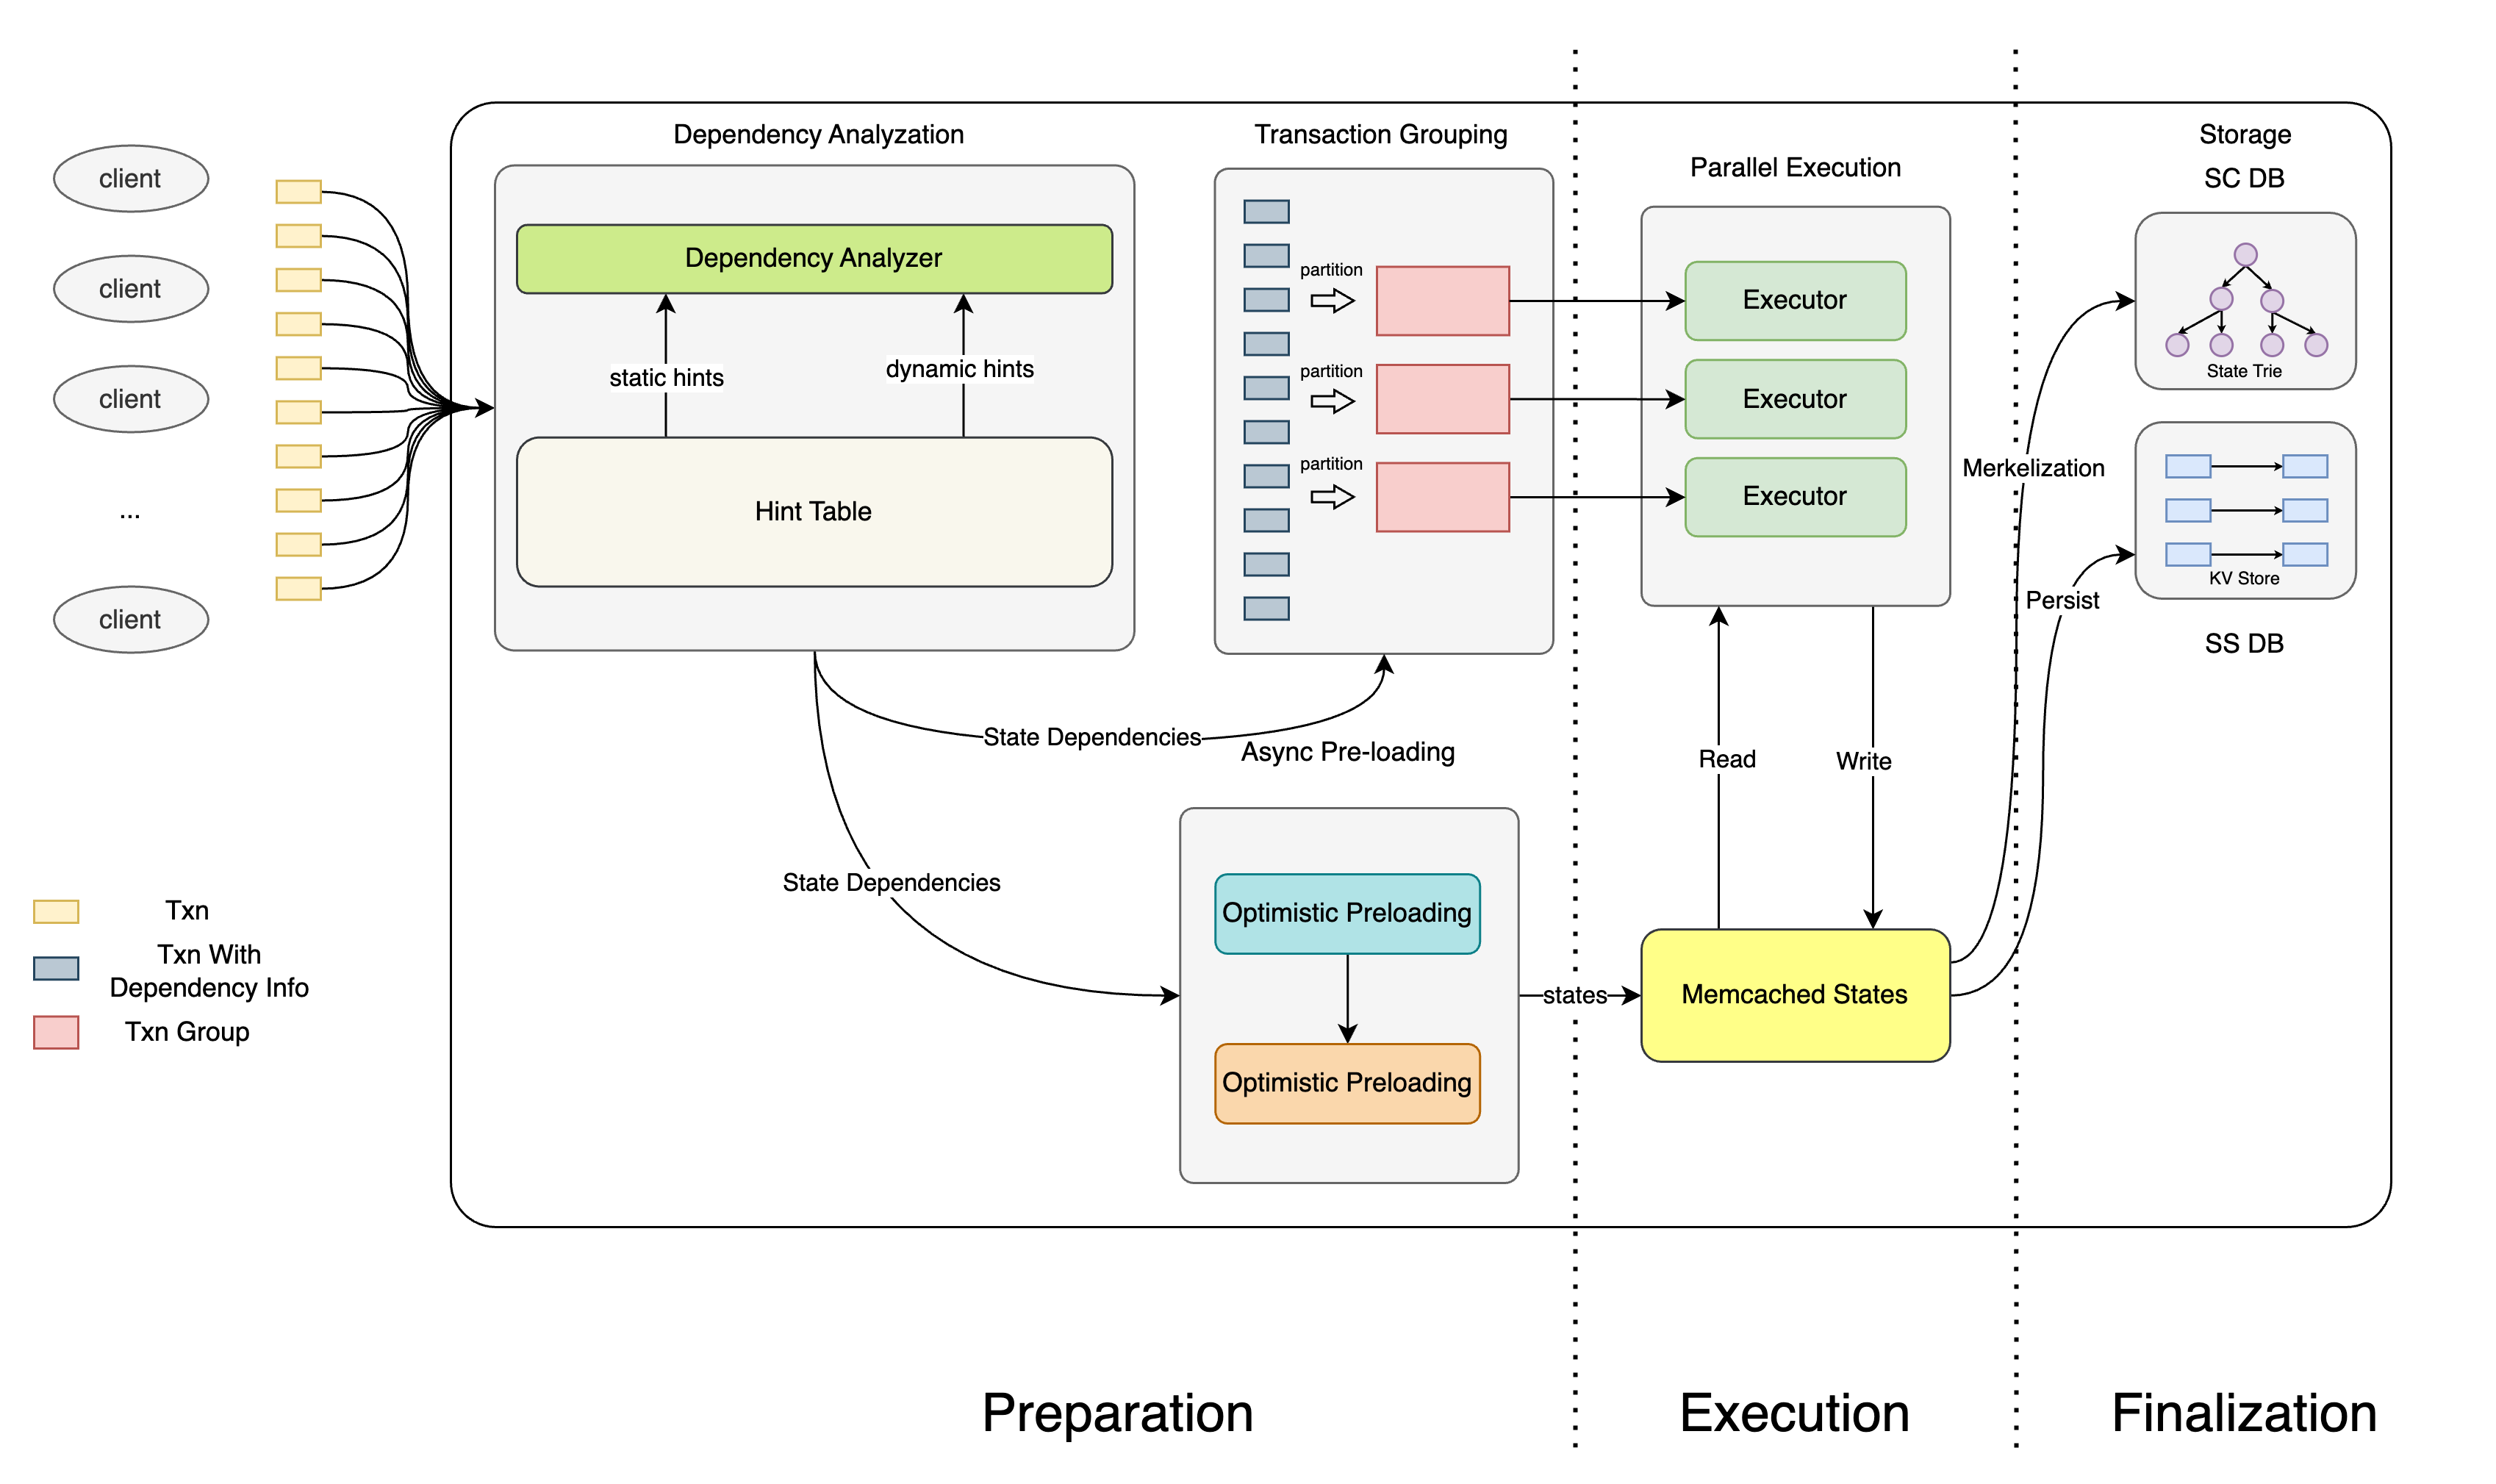
\includegraphics[width=0.75\textwidth]{sections/images/predictive-optimistic-execution.png}
\caption{Predictive Optimistic Execution}
\label{fig:predictive_optimistic_execution}
\end{figure*}

\subsection{Optimistic Execution}

Our algorithm employs "Optimistic Execution," a strategy where transactions are processed speculatively, operating under the initial assumption of conflict absence. Each transaction maintains a private version of the state, recording modifications without immediate finalization. Upon completion of the transaction, a subsequent validation phase examines for potential conflicts against global state alterations effected by concurrent transactions within the same interval. Any detected conflicts result in the abortion and re-execution of the transaction. 

This approach leverages a multi-version data structure and upholds a pre-defined serialization order to ensure data consistency and integrity. The refinement of the optimistic execution algorithm will be integrated through enhancements in BlockSTM.

\subsection{Hint table}

In this section, we will discuss the current challenges associated with existing hint resolution methods and discuss how \textbf{Artela's Hint Table} addresses these issues through its implementation.

\textbf{Hint Table} serves as an auxiliary database table. It is \textbf{persisted on the hard drive} and will be \textbf{preloaded into memory} prior to usage. The hint table cataloges potential transaction and contract read / write sets. This aids the division of transactions into parallel executable groups before execution, significantly reducing the conflict rate and re-execution times.

We will now discuss the current solutions similar to hint table and explain why they are inadequate for parallel execution needs.

\textbf{EIP-2930 (Optional Access Lists).} EIP-2930 introducing the ability for users to submit their transactions' read and write sets, but since this is not mandatory, only a small fraction of transactions are using it (\href{https://arxiv.org/html/2312.06574v1#:~:text=Analyzing%20a%20full%20month%20of,%24%205%20Mio)%20per%20year.}{1.46\%} until December 2023) utilize this feature.

\textbf{Transaction Pre-Execution.} Transactions are initially sent to pre-execution nodes (non-Validator nodes), where these nodes collect potential read-write sets through pre-execution, a method fundamentally employed by systems such as Sui due to its cost-effectiveness. However, this approach necessitates the addition of protocols between non-Validator and Validator nodes within the network.

\textbf{Static Analysis.} This approach utilizes a compiler or other tools to conduct static analysis and abstract interpretation, identifying the potential read-write sets that contract execution may access. These are analyzed in advance and stored as static hints. Along with the contract's bytecode, these hints are sent to nodes. Before executing the contract, nodes load these hints to enhance static analysis. A significant drawback of this method is the requirement for developers to adhere strictly to conventions. Sending invalid hints can lead to issues during algorithm execution.

The Hint table is engineered to adeptly address distinct challenges associated with discovering transaction and contract read/write sets by leveraging a combination of static and dynamic analysis. The following is a detailed explanation of its implementation and strategic approach to resolving these challenges.

\subsubsection{Types of States}

The hint table will categorize the states of contracts into the following categories:

\textbf{Input-unrelated States:} These states are universally accessible and generally easier to be analyzed, for example the `totalSupply` state variable in an ERC20 contract.

\textbf{Input-related States:} These states are dynamic; they are typically associated with transaction data.
\begin{itemize}
\item \textbf{Account-related States:} Directly connected to specific accounts, these states relate to transaction fields like \textbf{`tx.from`} and \textbf{`tx.to`}.
\item \textbf{Miscellaneous States:} These are dynamically linked states whose relationships are not consistently determinable, often seen in complex contracts like Uniswap V4's \textbf{`positions`} mapping.
\end{itemize}
\subsubsection{Types of Hints}

Hints can be categorized into two types:

\textbf{Static Hints:} This type signifies a basic hint, typically used to suggest actions for input-unrelated states. We can represent this type of hints with the following symbols:
    
    \begin{equation}
    \[
    C(M) \Rightarrow \{ R(slot_i), W(slot_j), ..., R(slot_k) \}
    \]
    \end{equation}

    $C$ represents a set of static configurations, when a smart contract method $M$ gets called, corresponding storage slot $slot_i$ will be read ($R$) / write ($W$).
    
\textbf{Dynamic Hints:} This type signifies the complex hint, typically used to suggest actions for input-related states. Dynamic hints can be represented with the following symbols:
    
\begin{equation}
\begin{split}
    F_i(M, \{a_i, a_j, ..., a_k\}) \Rightarrow \{ &R(slot_i), \\
    &W(slot_j), \\
    &..., \\
    &R(slot_k) \}
\end{split}
\end{equation}
    
    This notation describes a more complex hint. Specifically, a given contract method $M$ has one or more input parameters that include accounts (denoted as $a$). The set ${a_i, a_j, ... , a_k}$ can be determined through a derivation algorithm $F_i$, which calculates the storage slots $slot_i$ accessed during the method's execution.
    
    Formed by analyzing historical execution data, dynamic hints adapt over time, enhancing their precision and relevance to current conditions.

\subsubsection{Hint Generation Process \& Format}

During transaction execution, the hint generation module captures and logs state accesses and contract calls for each method and contract address. 

Hints are structured in a key-value format where the key represents a combination of fields, and the value denotes a set of state slot indices. For input-related states, hints don’t log every storage slot but use a mapping function to represent them efficiently.

\subsubsection{Storage of Hints}

To ensure operational efficiency, hints are stored persistently but loaded entirely into memory when accessed. The total size of stored hints is capped at under 4GB to optimize memory usage and maintain system performance.

This comprehensive overview delineates the structure, generation, and utilization of hints within the system, which are integral to optimizing contract interactions and enhancing transaction processing efficiency. By categorizing and systematically managing hints, the system ensures high levels of accuracy and operational efficacy.

\subsection{AI-driven Hints Generator}

Unlike other solutions that require developers to predefine hints, the Hint table does not need to be manually generated by developers. It supports the introduction of a specific AI model to analyze the execution of past historical transactions and automatically generate an accurate Hint table. Therefore, transactions on the Artela blockchain cannot be executed with a high degree of parallelism from the start; there will be a warm-up process. As the Hint table is gradually refined, the parallelism of the chain will automatically improve.
% sections/03-async-preloading.tex

\section{Async preloading}

To maximize the use of the CPU's concurrent computational capabilities and prevent I/O from becoming the execution bottleneck, we propose ``Async Preloading'', which is based on a predictive algorithm. This approach proactively preloads the states required for transaction execution into memory beforehand, thereby eliminating the need for I/O access during transaction execution.

The performance of a block is contingent on its slowest batch, which may suffer from higher computational demands or extended ``waiting'' times, primarily from disk reads for accounts and storage slots. Advanced predictive algorithms address computational bottlenecks by offering relatively optimal solutions, while I/O delays are mitigated through Async Preloading combined with the hint table, enhancing overall system performance.

The working process of async preloading is illustrated in figure \ref{fig:async_preloading}

\newpage

\begin{figure}[htp]
  \centering
  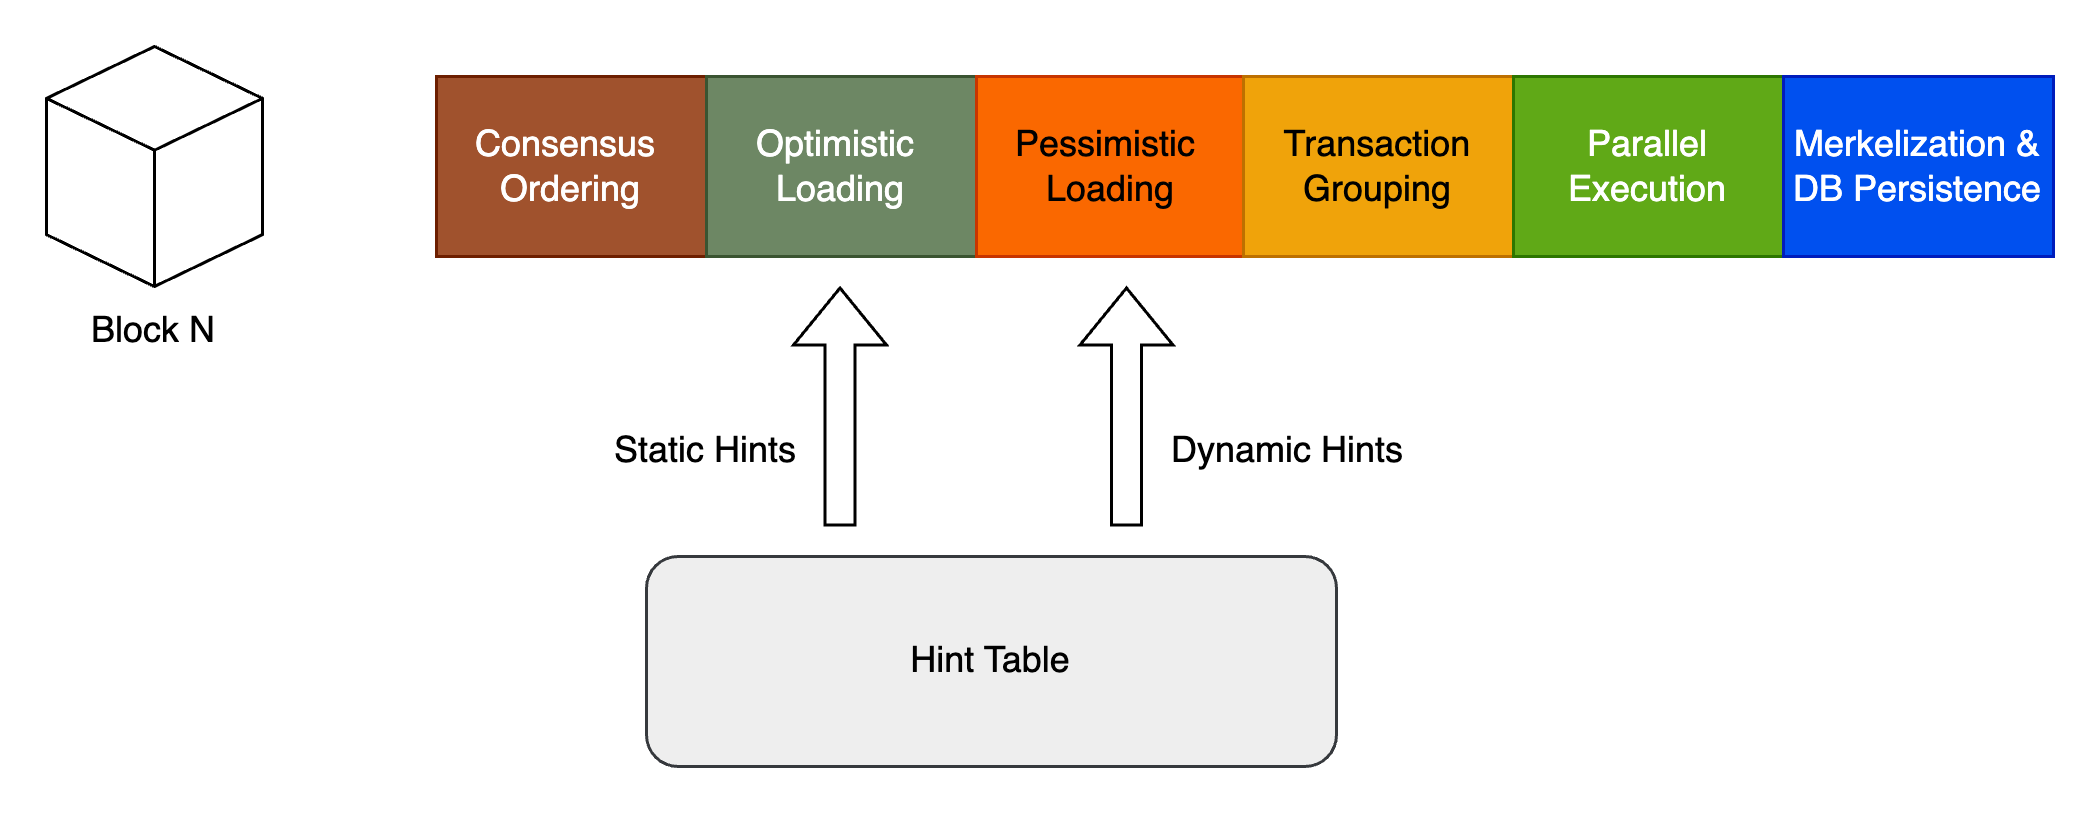
\includegraphics[width=0.5\textwidth]{sections/images/async-preloading.png}
  \caption{Async Preloading Process}
  \label{fig:async_preloading}
\end{figure}

Before executing the transaction, \textbf{Optimistic Preloading} is initiated, loading only the specified storage into memory according to static hints.

Following Optimistic Preloading, \textbf{Pessimistic Preloading} commences, loading all potential storage into memory in accordance with dynamic hints.

After completing the async preloading, all the necessary state storage is loaded into memory. Subsequent execution will be entirely based on memory, which is expected to enhance I/O performance by a factor of \textbf{10 to 1,000 times}.

\subsection{Optimistic Preloading}

When the transaction order is established within a single block, Optimistic Preloading assesses the essential key-values (KVs) of a smart contract and preloads the storage slots using static hints. This preloading process does not necessitate waiting for the transaction execution and can proceed asynchronously. The objective is to minimize I/O costs for each batch by ensuring that the necessary data is readily accessible. However, it is important to note that while optimistic preloading loads all the required storage slots, there may be misses. These misses will be addressed by pessimistic preloading.

\subsection{Pessimistic Preloading}

Following the completion of pessimistic preloading, pessimistic preloading employs a probabilistic model to predict which key-value pairs might be needed in upcoming transactions. This prediction, bolstered by Dynamic Hints, uses method signatures and call data to estimate potential read/write sets. Although these predictions may occasionally overestimate the needed data—due to transactions terminating early or other factors—this strategy aims to reduce execution times for each batch by utilizing additional I/O resources preemptively.
\section{Parallel storage}

The parallel storage is designed to address the final two performance challenges encountered in blockchain execution: enabling parallelizable storage and enhancing the efficiency of persisting Merkelized world states into a database. By parallelizing storage, it aligns with the parallel execution capabilities, effectively leveraging multi-core processing benefits. As historical data accumulates, the storage layer faces escalating issues related to write amplification and compaction, which can significantly degrade Merkelization performance.

When transactions are executed in parallel, multi-core processing is utilized effectively. However, if data persistence lags behind transaction execution, storage becomes a bottleneck, hindering blockchain performance. Parallelizable storage is essential for maximizing transaction parallel execution efficiency.

Merkelization performance pertains to the throughput and latency of writing Merkle tree-based world states into the database. The primary issues are write amplification and database performance. Each state modification requires the Merkle tree to re-encode and rewrite from leaf nodes to the root in the KV database. The KV database itself also experiences write amplification, leading to significant overhead. As data accumulates, the Merkle tree depth increases, resulting in more key-value pairs being written. This intensifies database background activities such as compaction, which consume substantial disk and CPU resources. Consequently, the throughput and performance of writing world states degrade significantly.

The parallel storage serves as an optimized storage solution specifically engineered to augment the efficiency of state storage within the Cosmos SDK. This layer is crafted to ensure seamless compatibility with established Cosmos storage frameworks, such as LevelDB or RocksDB, as well as the IAVL trie\cite{cosmos_iavl}\cite{simmon_avl_trees}, while introducing a substantially enhanced storage strategy. Notably, the existing implementation of Cosmos IAVL storage suffers from performance degradation as the blockchain state expands.

This layer addresses these challenges by optimizing I/O performance for extensive state manipulations and expediting the Merkelization process. It aims to rectify prevalent storage inefficiencies through a series of critical enhancements:

\begin{enumerate}
    \item Separation of State Commitment (SC) and State Storage (SS)
    \item K-Persist State Commitment Database
\end{enumerate}

\subsection{Separation of State Commitment and State Storage}

To achieve parallelizable storage, we have implemented a separation strategy between "State Commitment" (SC) and "State Storage" (SS). This approach allows us to distinctly categorize operations into parallelizable and non-parallelizable segments, enhancing system throughput and efficiency.

The storage architecture is organized as follows (shown in figure \ref{fig:sc_ss_separation}):

\begin{figure}[htp]
    \centering
    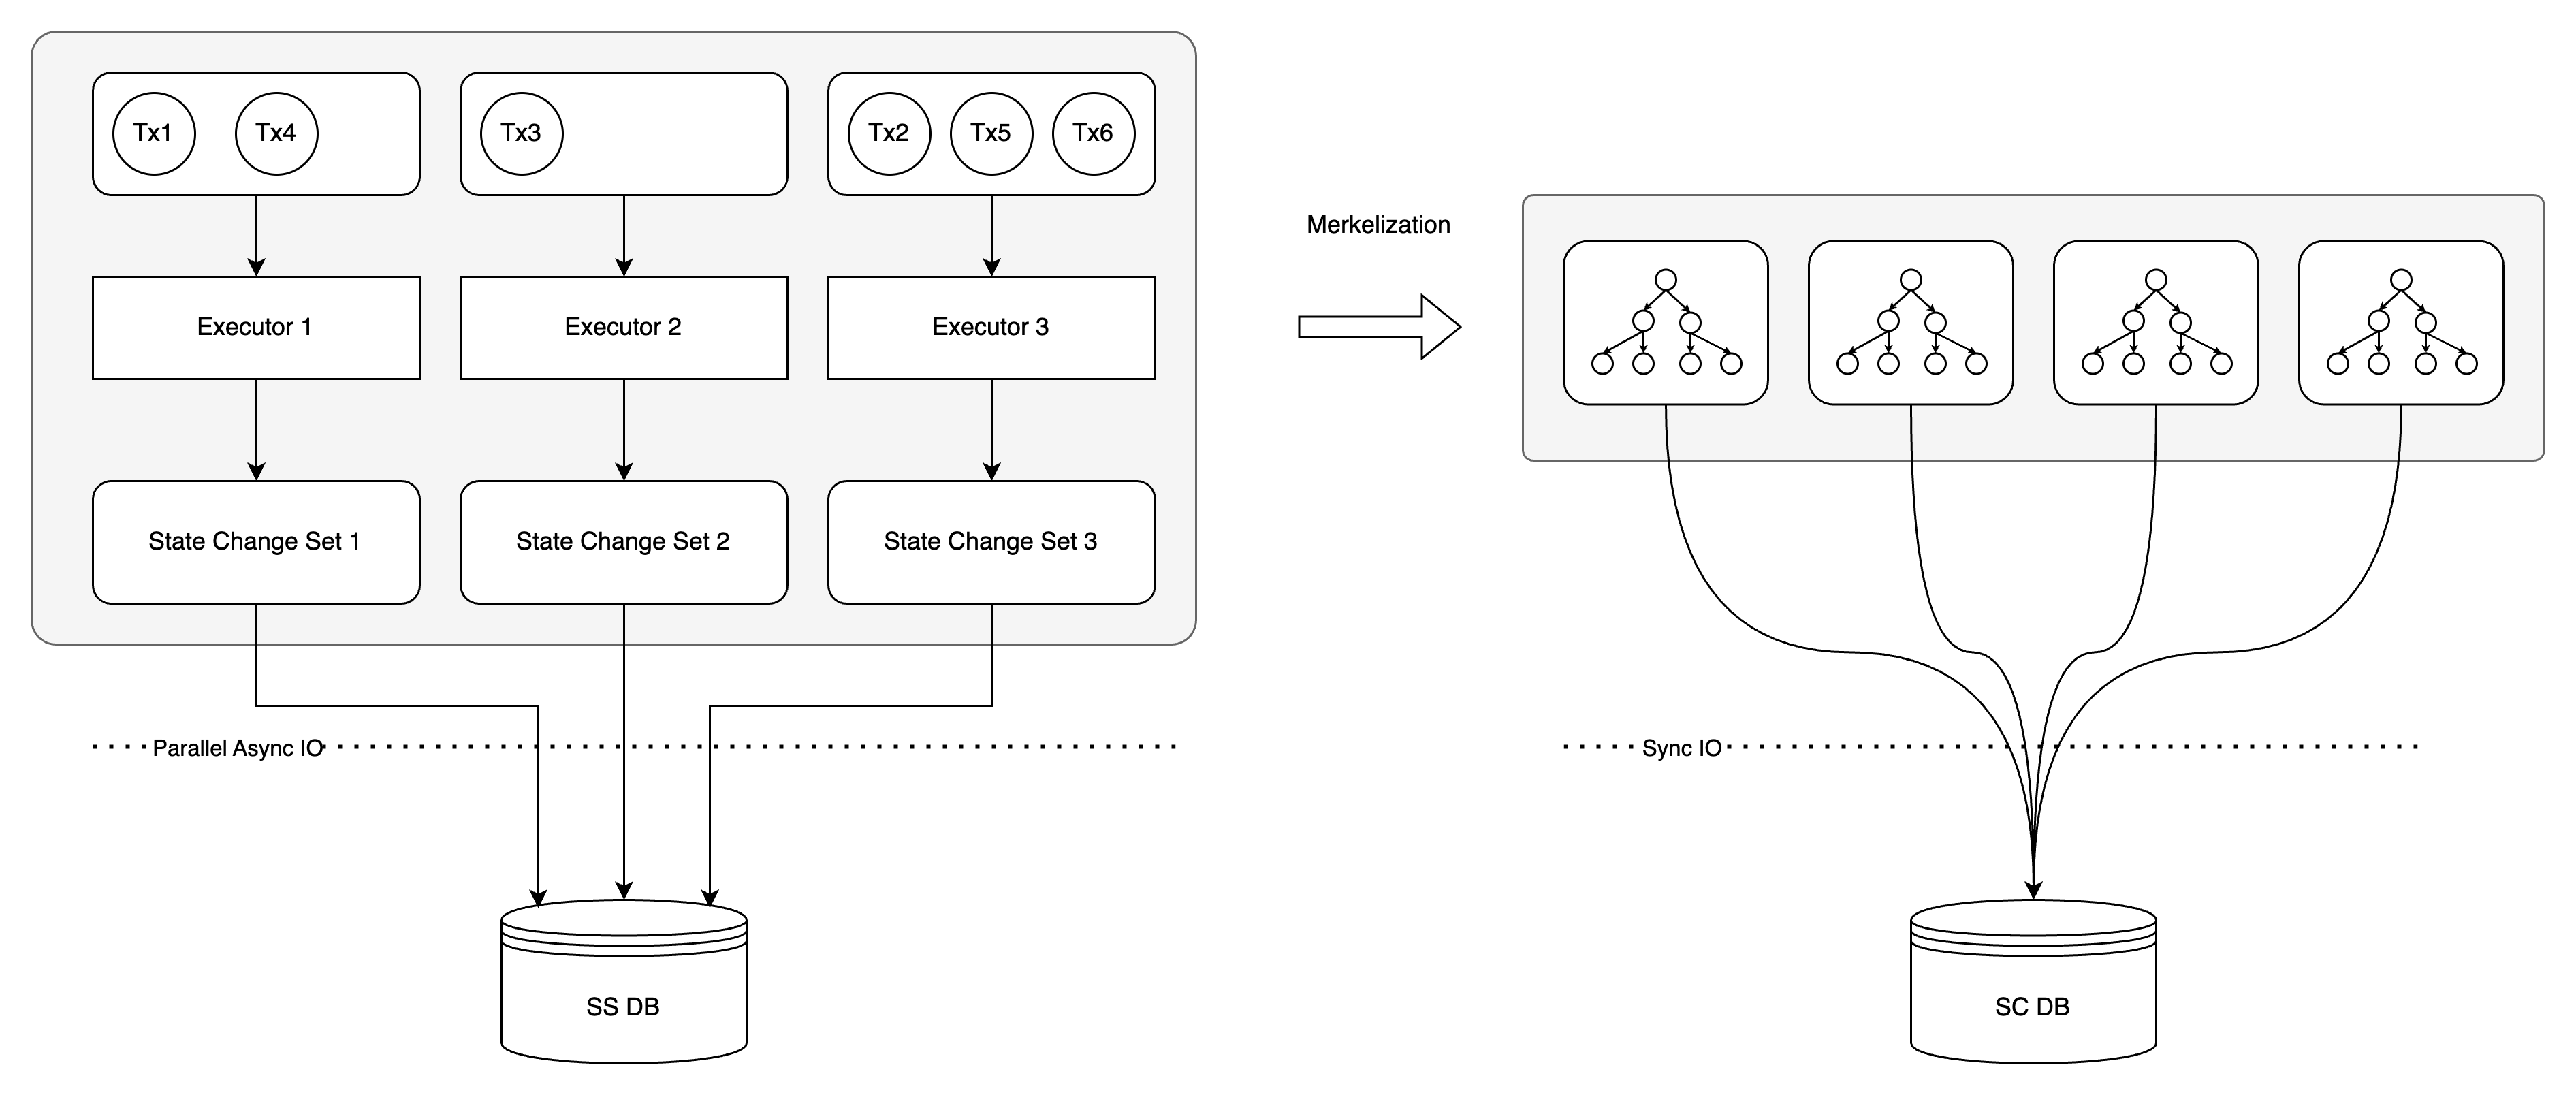
\includegraphics[width=\columnwidth]{sections/images/sc-ss-separation.png}
    \caption{Storage architecture}
    \label{fig:sc_ss_separation}
\end{figure}

\begin{itemize}
    \item SS DB is parallelizable and allows for asynchronous IO. It stores meta-information such as accounts and storage slots but does not retain any trie data. This approach prevents data redundancy and optimizes space utilization.
    \item SC DB is serial and uses synchronous IO. It records all trie information. Here, the leaf nodes retain only the hash information of accounts and storage slots, eschewing meta-information to avoid redundancy and streamline storage.
\end{itemize}

The design operates as follows:

\begin{itemize}
    \item Once transactions are grouped by parallelization criteria, an async preloading mechanism triggers parallel asynchronous read operations to SS DB. This is aimed at maximizing disk IOPS and bandwidth.
    \item Once the execution of a transaction group has finished, the results of each execution group are directly written to disk.
    \item Disk writing operations and Merkelization processes run concurrently without interference. The former utilizes I/O resources, while the latter depends on CPU resources. During this phase, the modification set is transferred to SC DB to obtain the State Root and generate the Block Header.
\end{itemize}

To reduce compaction and improve performance of merkelization, SS DB's storage is composed of four database instances:

\begin{itemize}
    \item Index DB: This database maps new addresses on the chain, converting 20-byte addresses into a 5-byte sequence to compress space, especially in databases like RocksDB/LevelDB that support prefix compression. Newly created addresses, likely to be active on the chain, are encoded in big-endian sequence. This positioning facilitates efficient querying as larger sequences are positioned towards the top of the database file.
    \item Account DB: records information from sequence to account, where sequence is encoded in big-endian.
    \item ContractDB: tracks information from sequence + storage slot to storage slot value.
    \item Write Set DB (Optional): Considering the different roles of Validators and Full Nodes in the network—Validators focus on consensus and transaction execution, while Full Nodes provide RPC services—special scenarios like SPV and State Sync require additional logging of each block's modifications in WriteSet DB.
\end{itemize}

This architecture effectively reduces the conflicts and resource wastage due to compaction in traditional LSM database designs, enhancing transaction execution efficiency by more than 60\% as demonstrated in benchmarks.

\subsection{K-Persist SC Database}

The following proposal outlines a universal persistent database design that supports more efficient Merkelization and the capability for multi-version data and SPV queries without compromising hash compatibility. 

The main idea is to aggregate multiple small-sized nodes of a Merkle tree into a larger-sized node for persistence, shortening the IO path, reducing write amplification, and decreasing space usage. Additionally, this approach leverages disk characteristics to achieve high-performance read and write operations. This type of persistent node is called a k-layer node. It draws on the design principles of Bw-tree to optimize the efficiency of world state persistence. This involves batch updates and deferred writes, combining multiple small write operations into a single larger write operation, thereby reducing the number of writes and improving write efficiency. 

Compared to 16-ary Merkle Patricia Tries (MPT) \cite{ethereum_patricia_merkle_trie} or Sparse Merkle Trees (SMT) \cite{fichter_sparse_merkle_tree}, binary structures like the IAVL exhibits significant read and write amplification issues. The deeper logical depth of binary trees, as opposed to 16-ary trees, results in more frequent disk I/O operations, which can become a critical issue during Merkelization.

The suboptimal performance of binary or even 16-ary Merkel Trees in blockchain systems is significantly due to frequent disk accesses, which increase the cost of read operations and thus create bottlenecks in the execution layer. This issue also poses one of the major shortcomings for Parallel EVM and Merkelization processes.

Considering that traditional hard disk sectors are typically 512 bytes, but modern drives—especially solid-state drives (SSDs)—feature a sector size of 4KB, we can leverage this characteristic for efficiency. Given that Merkel Trees in blockchain contexts are generally sparse, it's feasible to adjust the parameter $k$ so that $2^k$ nodes are compressed into a single minimal read/write unit, optimally around 3-4KB.

To maximize disk and I/O resource utilization for a Merkel Tree, each $k$-layer read/write operation is designed as follows:

\begin{enumerate}
    \item Load the Root Node: Based on the block number, load the root node where the World State Root resides.
    \item Merkelization Process: If Merkelization is necessary, load the corresponding Merkel Path's internal and leaf nodes according to the Write Set.
    \item Node Updates: Update the leaf nodes along the Merkel Path from the bottom up to compute the new root hash value. Mark this node as dirty and tag the corresponding $k$-layer nodes along the Merkel Path as dirty.
    \item Persistence of $k$-Layer Nodes: After computing the hash values, all $k$-layer nodes are persisted. The traditional Merkel node's primary bottleneck lies in its indexing information being hash values, which perform poorly in LSM databases. To circumvent this, we use the following encoding scheme to record all $k$-layer nodes:
    \begin{equation}
      \[
      B + D + S = K
      \]
    \end{equation}
      In this context, $B$ represents the block number, $D$ denotes the depth of the $k$-layer node, $S$ indicates the sequence number, and $K$ is the encoded key. All numbers are stored in big-endian format to ensure compatibility with compaction processes.
      Depth refers to the depth of the $k$-layer node and sequence is an incremental unique index, the layout of $k$-layer node is shown as the figure \ref{fig:k_persist_layer_node} illustrates.

      \begin{figure}[htp]
        \centering
        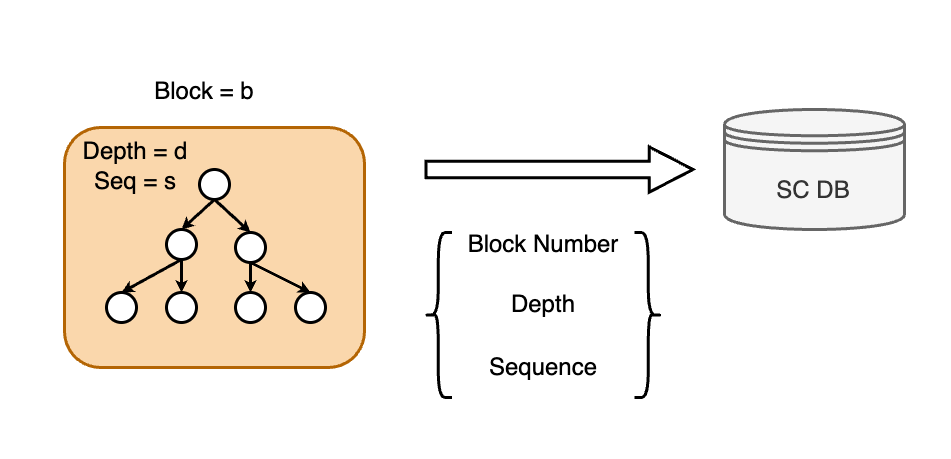
\includegraphics[width=\columnwidth]{sections/images/k-persist-layer-node.png}
        \caption{K-Persist Layer Node}
        \label{fig:k_persist_layer_node}
    \end{figure}
\end{enumerate}

To better delineate the parent-child relationships among $k$-layer nodes, inspired by traditional database systems such as RocksDB and InnoDB, we record the following details in each parent $k$-layer node for all its child $k$-layer nodes (up to $2^k$ nodes):

\begin{enumerate}
    \item Version: The version value of each child $k$-layer node at the time of its last modification.
    \item Sequence Number: A unique identifier for each child node.
    \item Start Key and End Key: These keys define the range of data that each child node covers.
\end{enumerate}

While typical search trees, like in the IAVL, inherently contain start key and end key information within each node, the K-Persist SC Database is designed to address their persistence challenges. Consequently, when $k$ is chosen to be relatively large, there is a potential scenario where $2^k$ nodes exceed the 4KB sector size limit, escalating to sizes such as 40KB or even 400KB. Such sizes would make read-write operations less efficient.

To navigate this dilemma, we may adopt a split and merge design strategy (shown in figure \ref{fig:k_layer_node_merge_split}). This would allow us to divide a large $k$-layer node into multiple smaller $k$-layer node and vice versa. It is important to note that:

\begin{figure}[htp]
    \centering
    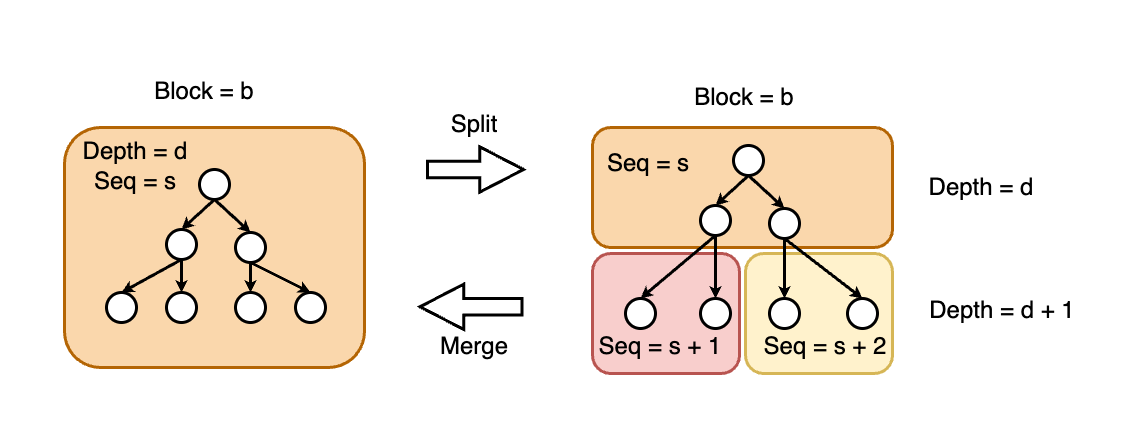
\includegraphics[width=\columnwidth]{sections/images/k-persist-layer-merge-split.png}
    \caption{K-Layer Node Merge and Split}
    \label{fig:k_layer_node_merge_split}
\end{figure}

\begin{itemize}
    \item Depth Consistency: The split $k$-layer node still retain the original depth $d$, as the value $k$ remains unchanged in the definition of each node.
    \item Node Design: The structure of $k$-layer nodes are similar to the design seen in MySQL's InnoDB\cite{mysql_innodb_architecture}, where nodes are part of a B+ tree. This means that like InnoDB, our design involves a bottom-up construction process, but adapted to our specific context with the added complexity of managing the Merkel-based blockchain data.
\end{itemize}

By integrating this adaptive split and merge capability, the K-Persist SC DB can dynamically adjust to the size requirements of the data it stores, ensuring efficient use of storage space and maintaining optimal performance even under varying load conditions. This approach not only enhances the flexibility of the database but also ensures scalability and efficiency in handling large-scale blockchain data.
\section{Elastic Block Space}

This proposal delineates a comprehensive strategy for implementing an \textbf{Elastic Block Space} (EBS) system within the Artela blockchain ecosystem. EBS refers to a dynamically scalable block space that provides independent and protocol-guaranteed block space for dApps with high transaction throughput needs, ensuring predictable performance. By introducing EBS, Artela endeavors to overcome the constraints of fixed block space capacity, enabling seamless scalability while maintaining predictable performance and efficient resource utilization.

Typically, a monolithic blockchain or an execution layer has only one shared block space available for all dApps, which may lead to the competition between different dApps causing unpredictable gas fee and performance. For dApps with high traffic and a high number of on-chain interactions, competition for block space greatly damages user experience. Opting for app chains or rollups to obtain independent block space introduces significant development burdens and a loss of composability. In Artela, EBS provide a solution to address this dilemma. When a dApps needs more performance predictability, it can apply for  dedicated block space. This additional space is integrated into the block and is exclusively used for the dApp's transactions. As block space increases, validators must scale "up" by adding elastic execution nodes to handle the enhanced processing load.

Elastic block space is a pivotal blockchain scaling mechanism, facilitating limitless scalability while ensuring interoperability. Unlike other scalable networks such as sharded blockchains, app chain networks, and Layer 2 solutions—which provide independent block spaces but suffer from isolation and unsynchronized block generation—elastic block space enables dApps with dedicated block spaces to conduct synchronous interactions through atomic transactions within the same block, circumventing the complexities of asynchronous cross-chain communications.

When a dApp in the Artela network demands high scalability, it can subscribe to elastic block space to manage the increase in transaction volume. This functionality, combined with native extensions, grants dApps on Artela enhanced scalability and customization potential.

\subsection{Block Space Type}

\begin{figure}[htp]
\centering
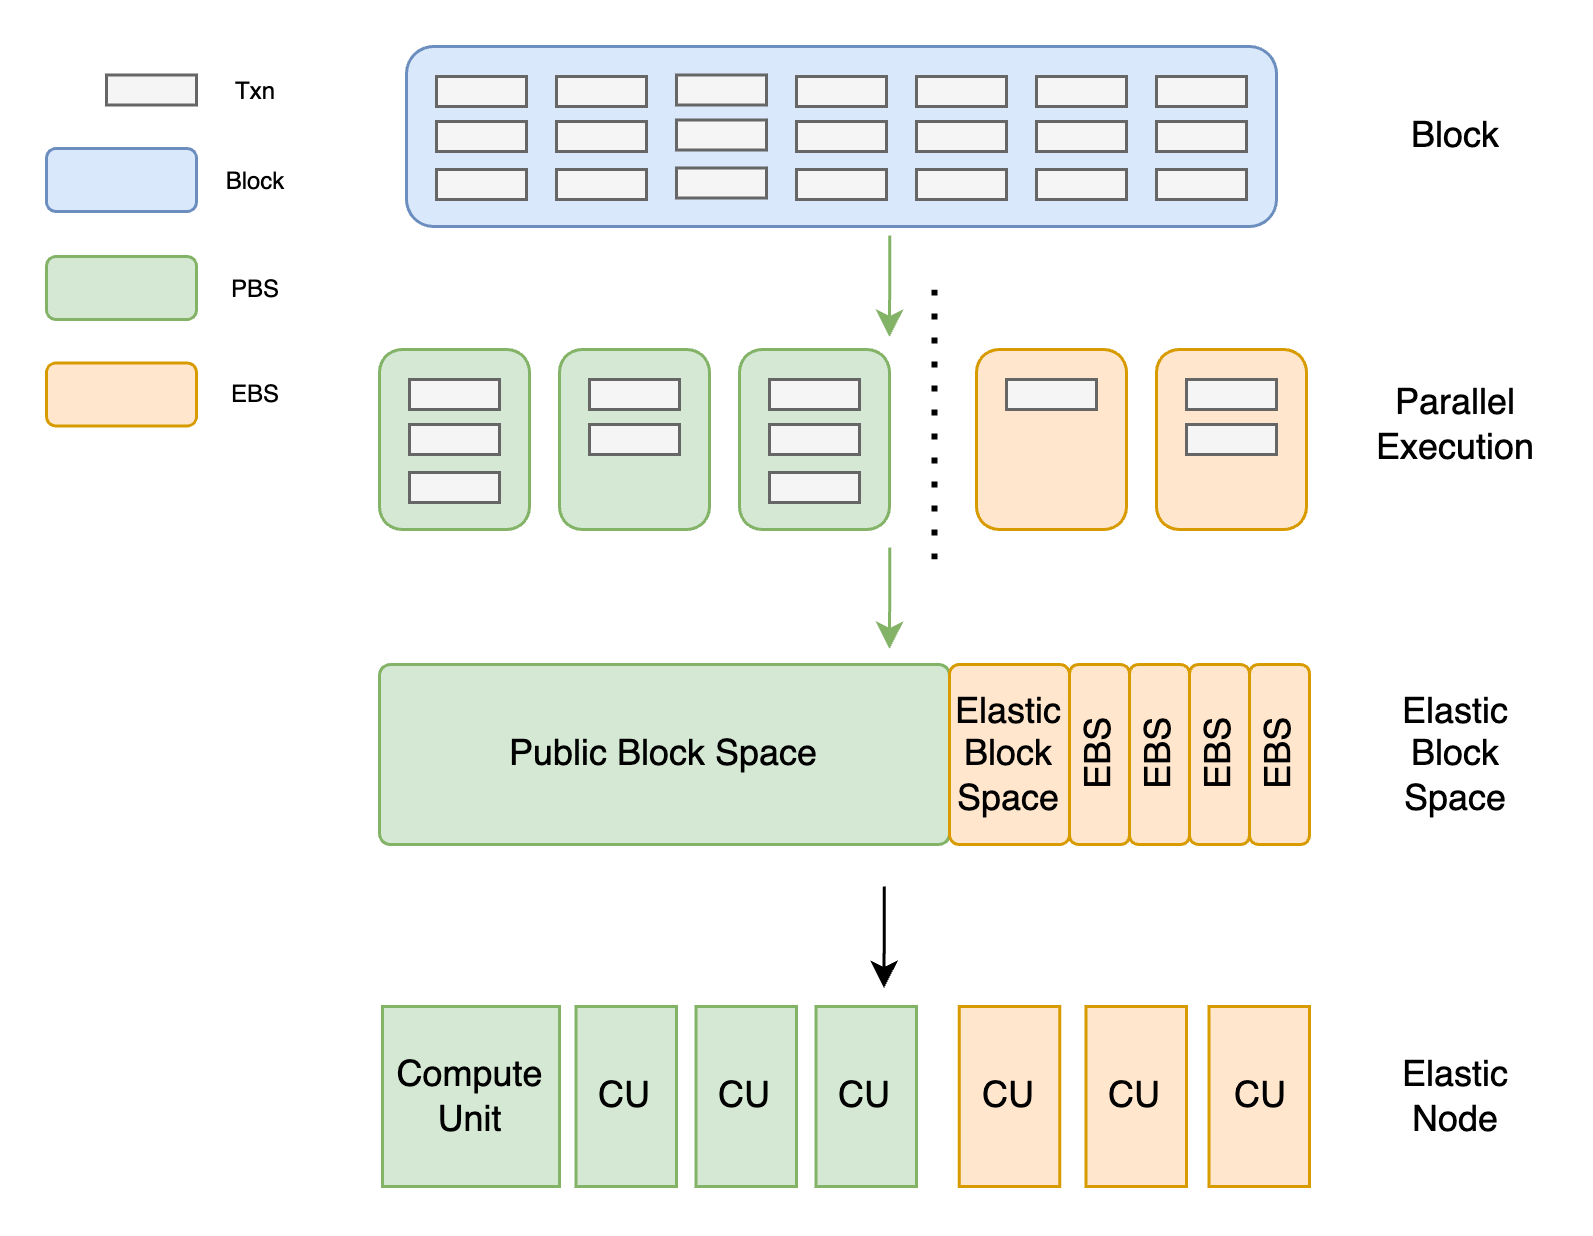
\includegraphics[width=\columnwidth]{sections/images/elastic-block-space.png}
\caption{Block Space Type}
\end{figure}

\textbf{Public Block Space.} Traditionally, blockchain blocks have been restricted by a fixed public block space (PBS) capacity. Transactions within PBS must vie for block space using gas fees, potentially leading to congestion and heightened transaction fees during periods of high network activity.

\textbf{Elastic Block Space.} Elastic Block Space introduces a dynamic block space allocation mechanism enabling dApps to request dedicated block space as necessary. This additional space is seamlessly integrated into the block and exclusively reserved for the transactions of the requesting dApp.

\subsection{Elastic Block Space}

WWhen a dApp in the Artela network requires high scalability, it can opt for elastic block space to manage the increase in transaction volume.

Elastic Block Space provides dApps with dedicated and protocol-guaranteed block space tailored to their transaction throughput requirements. This mechanism confers several key advantages:

\begin{itemize}
\item \textbf{Subscription Model:} DApps can sign transactions to dynamically subscribe to the elastic block space services. This implementation allows dapps to utilize chain-level independent block space without any additional development related to blockchain infrastructure.
\item \textbf{Independent Block Space:} dApps can request additional block space to accommodate high transaction volumes, dedicated for its own usage. Validators scale up by adding elastic execution nodes to manage the augmented load. Independent block space is limited by gas but measured by execution time; the better parallelization the contract can achieve, the larger gas limit this block space will have.
\item \textbf{Interoperability:} In contrast to sharded blockchains or app chain networks, which often encounter challenges with asynchronous cross-chain communications, elastic block space enables synchronous interactions via atomic transactions within the same block. This ensures seamless integration and native composability for dApps operating within the same blockchain.
\end{itemize}

\subsection{Elastic Node}

Artela's validator nodes are structured as an Elastic Cluster, supporting dynamic scaling through the addition or removal of execution nodes as required. Each EBS will be allocated a dedicated CU to execute its transactions. This cluster architecture is underpinned by the following core concepts:

\begin{itemize}
\item \textbf{Compute Unit (CU):} This serves as a fundamental execution module with a fixed number of CPU cores, capable of parallel computation with predictable transaction processing throughput (TPS). Each CU can manage multiple parallel execution groups.
\item \textbf{Basic CUs:} These constitute the minimum configuration for an Artela validator node, ensuring a baseline level of TPS for the network.
\item \textbf{Stepwise Scaling:} The network can dynamically scale by adding or removing CUs based on average load. For instance, if the load exceeds 125\% of the current capacity, a proposal can be initiated to increase the number of CUs. Once the proposal is approved, the network can scale up and reduce the overhead. Conversely, if the load drops below 25\%, a proposal can also be made to reduce CUs. Scaling decisions are governed by consensus among nodes.
\item \textbf{Subscription Scaling:} As supplementary to stepwise scaling, CUs can also be dynamically scaled upon EBS subscription. When a new EBS is subscribed to, a dedicated CU will be assigned for executing the transactions within the given EBS.
\end{itemize}

\subsection{Predictable Performance of EBS}

Artela's \textbf{Elastic Block Space} ensures predictable performance for decentralized applications (dApps) by providing dedicated block space and elastic computing power that scales according to demand. The gas mechanism, initially proposed by Ethereum as an innovative way to measure the resource consumption of smart contracts, can be expressed through the following equation:

\begin{equation}
G \equiv C(x) + M(y) +  S(z)
\end{equation}

Here, $G$ represents the gas cost, $C$ denotes the conversion function for CPU time to gas, $M$represents the conversion function for memory usage to gas, and $S$ stands for the conversion function for storage usage to gas.

However, this approach is not applicable to EBS with parallel execution enabled. For EBS + parallel execution, a new measuring model will be applied, which is:

\begin{align}
t_\text{pbs} &\equiv F(g_\text{pbs}) \\
g_\text{ebs} &\equiv G( t_\text{pbs}  \times P) 
\end{align}

$g_\text{ebs}$ represents the gas limit of the EBS. A function $F$ will convert the gas limit of PBS ($g_\text{pbs}$) to the execution time $t_\text{pbs}$, multiplied by the parallelism of the given dApp $P$ to obtain the maximum allowed execution time of this EBS. After that, by applying a conversion function $G$, the given execution time will be converted to the gas limit of EBS.

Initially, the parallelism $P$ of the given dApp cannot be determined, so the initial $g_\text{ebs}$ will be set to a fixed value $t_\text{block} / 1000000$ (assuming 1 second of CPU execution equals to 10 million gas, the same assumption as Ethereum’s). This value is for the worst-case scenario, meaning if a dApp cannot be parallel executed at all, at least the EBS can have this much gas limit (without affecting the execution time of the entire block). As more transactions are executed, the parallelism $P$ will be better estimated. The estimation of $P$ will be determined by the following equation:

\begin{align}
U &\equiv g_\text{used} / g_\text{ebs} \\
I &\equiv (t_\text{pbs} - t_\text{ebs}) / t_\text{pbs} \times U \\
P_\text{new} &\equiv P_\text{old} * (1 + I)
\end{align}

Here, $U$ represents the usage level of the EBS. $I$ represents the change of parallelism from the last block, calculated from the execution time differences between PBS and EBS with gas usage level applied for a relatively accurate change in parallelism from the block. By continually adjusting the parallelism parameter, the gas limit of EBS can converge to an optimal value, thereby making its execution time more predictable and maximizing the computing power usage of the CU.

\subsection{Governance and Scaling}

The operational framework of the elastic block space relies on governance mechanisms and dynamic scaling strategies aimed at optimizing resource allocation and ensuring network efficiency. To ensure the scalability of resources for the elastic block space at the protocol level, the following methodologies will be employed:

\begin{itemize}
\item \textbf{Staking Scaling:} Access to virtual block space necessitates dApps to stake a specific quantity of tokens. This action initiates node expansion, thereby furnishing dedicated resources for the dApp’s smart contracts. An auction mechanism with low entry barriers ensures equitable access and allocation of resources.
\item \textbf{Dynamic Node Management:} The elastic node architecture facilitates dynamic scaling, which is governed by network consensus protocols. This mechanism empowers validators to scale resources up or down in response to real-time demand, thereby upholding optimal performance and resource utilization.
\end{itemize}

In summary, Artela's Elastic Block Space and Elastic Cluster offer a robust framework for scalable and predictable blockchain performance, ensuring that dApps can operate efficiently and effectively irrespective of transaction volume. This innovative approach amalgamates dynamic scaling with dedicated resources, providing a flexible and potent solution for the evolving needs of blockchain applications.
\section{Conclusion}

In this paper, we discuss the parallel execution stack, which enhances the scalability of the Artela blockchain and provides applications with predictable performance. It enhances the traditional EVM with features such as predictive optimistic execution and async preloading, which optimize parallel transaction processing and I/O performance. The fast persistent storage layer improves storage efficiency, while the elastic block space model allows decentralized applications to request dedicated block space, further boosting network efficiency. These innovations make Artela EVM++ well-suited for integrating advanced technologies and supporting a wide range of decentralized applications.
% \newpage

\bibliographystyle{unsrt}
\bibliography{references}
 

\end{document}
